% abtex2-modelo-artigo.tex, v-1.9.2 laurocesar
% Copyright 2012-2014 by abnTeX2 group at http://abntex2.googlecode.com/ 
%

% ------------------------------------------------------------------------
% ------------------------------------------------------------------------
% abnTeX2: Modelo de Artigo Acadêmico em conformidade com
% ABNT NBR 6022:2003: Informação e documentação - Artigo em publicação 
% periódica científica impressa - Apresentação
% ------------------------------------------------------------------------
% ------------------------------------------------------------------------

\documentclass[
	% -- opções da classe memoir --
	article,			% indica que é um artigo acadêmico
	11pt,				% tamanho da fonte
	oneside,			% para impressão apenas no verso. Oposto a twoside
	a4paper,			% tamanho do papel. 
	% -- opções da classe abntex2 --
	%chapter=TITLE,		% títulos de capítulos convertidos em letras maiúsculas
	%section=TITLE,		% títulos de seções convertidos em letras maiúsculas
	%subsection=TITLE,	% títulos de subseções convertidos em letras maiúsculas
	%subsubsection=TITLE % títulos de subsubseções convertidos em letras maiúsculas
	% -- opções do pacote babel --
	english,			% idioma adicional para hifenização
	brazil,				% o último idioma é o principal do documento
	sumario=tradicional
	]{abntex2}


% ---
% PACOTES
% ---

% ---
% Pacotes fundamentais 
% ---
\usepackage{lmodern}			% Usa a fonte Latin Modern
\usepackage[T1]{fontenc}		% Selecao de codigos de fonte.
\usepackage[utf8]{inputenc}		% Codificacao do documento (conversão automática dos acentos)
\usepackage{indentfirst}		% Indenta o primeiro parágrafo de cada seção.
\usepackage{nomencl} 			% Lista de simbolos
\usepackage{color}				% Controle das cores
\usepackage{graphicx}			% Inclusão de gráficos
\usepackage{microtype} 			% para melhorias de justificação
\usepackage{float}
% ---
		
% ---
% Pacotes adicionais, usados apenas no âmbito do Modelo Canônico do abnteX2
% ---
\usepackage{lipsum}				% para geração de dummy text
% ---
		
% ---
% Pacotes de citações
% ---
\usepackage[brazilian,hyperpageref]{backref}	 % Paginas com as citações na bibl
\usepackage[alf]{abntex2cite}	% Citações padrão ABNT
% ---

% ---
% Configurações do pacote backref
% Usado sem a opção hyperpageref de backref
\renewcommand{\backrefpagesname}{Citado na(s) página(s):~}
% Texto padrão antes do número das páginas
\renewcommand{\backref}{}
% Define os textos da citação
\renewcommand*{\backrefalt}[4]{
	\ifcase #1 %
		Nenhuma citação no texto.%
	\or
		Citado na página #2.%
	\else
		Citado #1 vezes nas páginas #2.%
	\fi}%
% ---

% ---
% Informações de dados para CAPA e FOLHA DE ROSTO
% ---
\titulo{Um estudo sobre soluções Blockchain\\ para segurança em Internet das coisas}
\autor{Gustavo Emanuel Kundlatsch}
\local{Universidade Federal de Santa Catarina}
\data{Março de 2019}
% ---

% ---
% Configurações de aparência do PDF final

% alterando o aspecto da cor azul
\definecolor{blue}{RGB}{41,5,195}

% informações do PDF
\makeatletter
\hypersetup{
     	%pagebackref=true,
		pdftitle={\@title}, 
		pdfauthor={\@author},
    	pdfsubject={Modelo de artigo científico com abnTeX2},
	    pdfcreator={LaTeX with abnTeX2},
		pdfkeywords={abnt}{latex}{abntex}{abntex2}{atigo científico}, 
		colorlinks=true,       		% false: boxed links; true: colored links
    	linkcolor=blue,          	% color of internal links
    	citecolor=blue,        		% color of links to bibliography
    	filecolor=magenta,      		% color of file links
		urlcolor=blue,
		bookmarksdepth=4
}
\makeatother
% --- 

% ---
% compila o indice
% ---
\makeindex
% ---

% ---
% Altera as margens padrões
% ---
\setlrmarginsandblock{3cm}{3cm}{*}
\setulmarginsandblock{3cm}{3cm}{*}
\checkandfixthelayout
% ---

% --- 
% Espaçamentos entre linhas e parágrafos 
% --- 

% O tamanho do parágrafo é dado por:
\setlength{\parindent}{1.3cm}

% Controle do espaçamento entre um parágrafo e outro:
\setlength{\parskip}{0.2cm}  % tente também \onelineskip

% Espaçamento simples
\SingleSpacing

% ----
% Início do documento
% ----
\begin{document}

% Retira espaço extra obsoleto entre as frases.
\frenchspacing 

% ----------------------------------------------------------
% ELEMENTOS PRÉ-TEXTUAIS
% ----------------------------------------------------------

%---
%
% Se desejar escrever o artigo em duas colunas, descomente a linha abaixo
% e a linha com o texto ``FIM DE ARTIGO EM DUAS COLUNAS''.
% \twocolumn[    		% INICIO DE ARTIGO EM DUAS COLUNAS
%
%---
% página de titulo
\maketitle

% resumo em português
\begin{resumoumacoluna}
  Segurança em Internet das coisas é uma questão em aberto no mundo acadêmico.
  Por conta da baixa capacidade computacional, baixa memória e baixo consumo de
  energia desse tipo de dispositivo, ter um software seguro rodando é algo que
  pode ser bastante difícil devido as limitações técnicas. 
  Neste artigo iremos discutir o que são os conceitos de Internet das coisas,
  segurança e blockchain, e revisar as soluções estado da arte da literatura
  que utilizam blockchain para segurança em internet das coisas. Será discutido
  os problemas atuais em aberto, as soluções mais modernas propostas e uma
  revisão dos trabalhos mais relevantes dessa área.
 
 \vspace{\onelineskip}
 
 \noindent
 \textbf{Palavras-chaves}: internet das coisas, blockchain, segurança.
\end{resumoumacoluna}

\section{Introdução}

Dentro da Inteligência Artificial (IA), agentes inteligentes são entidades capazes de raciocinar a respeito do ambiente em que estão inseridos e tomar decisões baseadas na situação em que se encontram \cite{russell2016artificial}. Dessa maneira, podemos descrever um agente pelo seus processos de percepção, raciocínio e atuação. O agente ocupa um ambiente, do qual recebe informações e no qual atua. O ambiente é o mundo em que o agente está inserido, podendo ser uma construção virtual como uma simulação ou uma parte do mundo real, no caso de um agente físico. Existem diversos tipos de ambientes que podem ser classificados de acordo com o seu fechamento (que determina se agentes de fora do ambiente podem afetar o sistema), dinamismo (a maneira como o ambiente evolui), determinismo (a consistência dos efeitos no ambiente) e cardinalidade (o número de objetos a serem afetados e percebidos) \cite{moya2007towards}.

Uma das maneiras de um agente atualizar seu conhecimento a respeito do ambiente é a percepção, o processo de utilizar sensores para detectar o ambiente e transformar os dados coletados em informações úteis \cite{weyns2004towards}.  O raciocínio, por sua vez, é o processamento das percepções baseado nos objetivos do agente, que resulta em um conjunto ações a serem tomadas através dos atuadores. O processo do raciocínio é comandado pela arquitetura cognitiva do agente, um modelo computacional inspirado na estrutura da mente humana \cite{DYACHENKO2018130}. As arquiteturas cognitivas podem ser divididas em três categorias: simbólicas, emergentes e híbridas \cite{yeCognitivearchitectures}. Arquiteturas simbólicas descrevem o ambiente através de símbolos armazenados em memória em uma base de conhecimentos, e utilizam lógica simbólica para realizar o ciclo de percepção, raciocínio e ação. Arquiteturas emergentes se baseiam na estrutura biológica do cérebro e normalmente utilizam redes neurais em uma estrutura hierárquica para lidar com situações de incerteza. Por fim, arquiteturas híbridas combinam o comportamento emergente e o processamento simbólico para resolver problemas de diversos domínios. 

Todavia, sensores podem apresentar problemas para o processo de percepção por razões como campo de visão, distância do objeto observado, resolução dos sensores e leituras não confiáveis \cite{chrisman1991intelligent}. Tratar deste problema normalmente é responsabilidade da arquitetura cognitiva do agente, pois a arquitetura precisa ser capaz de fazer a ponte entre o ambiente e o conhecimento do agente \cite{langley2009cognitive}.

O objetivo deste trabalho é apresentar um modelo genérico (independente da arquitetura do agente) que pode ser acoplado entre o processo de percepção e raciocínio, capaz de detectar e tratar percepções inválidas para transformá-las em informações úteis através de um processo de criação de novos planos. Esse modelo pressupõe um ambiente aberto (onde agentes externos podem influenciar o ambiente), dinâmico (mudanças no ambiente são causadas por eventos aleatórios) e não determinístico (ações do agente causam resultados diferentes no ambiente, mesmo em situações aparentemente idênticas, pois os resultados variam dependendo da percepção do agente daquele evento).  

\section{Conceitos básicos}

A seção de conceitos básicos é destinada a apresentar elementos fundamentais para a revisão bibliográfica proposta. No caso específico desse artigo, optamos por apresentar os seguintes três temas: Internet das Coisas, Segurança e Blockchain. Como esses são conceitos relativamente avançados de computação, é necessário garantir que eles sejam bem compreendidos para que tanto a revisão do estado da arte quanto a proposta de solução sejam bem sucedidos. Além de serem conceitos relativamente avançados de computação, eles também se comportam como blocos básicos para construir conceitos mais avançados. Por exemplo, como queremos mostrar as soluções de publicações atuais sobre o uso de Blockchain em Segurança, é preciso compreender a fundo o que é uma rede Blockchain para saber quais os benefícios mas também as desvantagens de tomar essa solução para resolver o problema de segurança em uma rede de Internet das Coisas.

\subsection{IoT}


Internet das Coisas, possuí uma carga teórica bastante pesada para ser profundamente compreendida. Apesar de seu conceito poder ser facilmente passado para o público leigo como ``as coisas do dia a dia conectadas a internet'' como máquinas de lavar roupa, cafeteiras, robôs de limpeza do chão ou até lâmpadas, seu conceito teórico envolve uma série de tecnologias de ponta que envolvem redes, dispositivos embarcados e, para nosso caso em especial, segurança. Um sistema embarcado (ou sistema embutido) é um sistema que possui um microprocessador e em que o computador é completamente ligado a computação do dispositivo que ele controla \cite{ganssle2003embedded}. Em computadores de propósito geral o sistema pode ser programado para fazer qualquer coisa que tenha capacidade técnica para realizar. Um sistema embarcado, por outro lado, realiza um conjunto de tarefas que foram predefinidas em sua confecção, com limitações tanto em hardware (componentes lógicas para tarefas específicas) quanto em software (programa dedicado ou sistema operacional compilado de acordo com a necessidade). A ideia de ter um sistema que realiza apenas um objetivo específico é a capacidade de otimização computacional, que reflete na capacidade de otimizar custo, gerando um preço muito melhor para o usuário final.

O conceito de internet das coisas está intimamente ligado aos sistemas embarcados, pois surge da junção de objetos do cotidianos, que a partir de uma placa embarcada consegue se conectar na internet \cite{iotDef} para realizar as tarefas necessárias, tanto para a otimização da própria tarefa que o objeto realiza quanto para conseguir uma boa performance em relação ao conjunto que o objeto compõem, como em uma casa inteligente em que todos os objetos se comunicam para agregar qualidade de vida aos moradores.

A internet das coisas é um conceito que não é novo, pois as empresas de tecnologia e especialistas discutem a ideia há décadas, sendo que a primeira torradeira conectada à internet foi revelada em uma conferência em 1989.
O ecossistema da internet das coisas (IoT) é composto por um
grande número de dispositivos interconectados que coletam, processam
gerar e compartilhar grandes quantidades de (possivelmente sensíveis e
informação critica \cite{brotsis2019blockchain}. Ou seja, IoT denota os dispositivos eletrônicos ou elétricos de muitos tamanhos e capacidades diferentes conectados à Internet \cite{miraz2018blockchain}.

Diversos objetos do nosso cotidiano podem ter suas versões conectadas a internet, como por exemplo eletrodomésticos, dispositivos médicos, câmeras, e todos os tipos de sensores. Isso abre as portas para inovações que facilitar novas interações entre os próprios objetos e os seres humanos, e pode abrir caminho para inovações ainda mais interessantes, como cidades inteligentes e carros autônomos. A crescente de objetos conectados a internet é resultado do barateamento da internet por si só, e também da popularização de dispositivos como smartphones, que torna concebível para o usuário final dispositivos ainda mais diferentes conectados a internet e se comunicando.
Um exemplo de como dispositivos IoT devem se tornar ainda mais presentes no futuro são os wearables, dispositivos inteligentes feitos para você vestir. O exemplo mais básico são os smartwatches, que no seu pulso são capazes de avisar sobre notificações recebidas no celular, batimentos cardíacos, dar informações detalhadas de GPS e outras diversas aplicações. Wearables ainda mais ousados como pulseiras, tênis e até bijuterias devem se tornar comum nas próximas décadas, por conta do seu custo relativamente baixo e miríade de aplicações.

\subsection{Segurança}

 Segurança é um tópico especialmente profundo, pois envolve desde coisas mais práticas e até simples (porém de uma grande base matemática) como a criptografia até conceitos mais complexos como ataques distribuídos ou injeções em programas desprotegidos. Segurança da computação certas vezes se torna até mesmo um tabu pela imagem negativa que tem sido continuamente passada pela mídia de \textit{hackers} e \textit{crackers}, programadores que utilizam seu conhecimento avançado em computação para realizar ataques danosos, seja por motivos pessoais como prestígio e crimes virtuais para estorquir ou roubar, ou por motivos mais autruístas como o \textit{cyber} ativismo. Apesar de ter esse conotação muitas vezes tomada como negativa, profissionais de segurança da informação trabalham justamente para evitar que pessoas mal intencionadas se aproveitem de falhas que passaram em branco tanto pela equipe de programação quanto pela equipe de testes de uma empresa.

A segurança da informação (SI) tem como objetivo proteger um dado conjunto de informações, como o próprio nome sugere, no sentido de preservar o valor que possuem para um determinado indivíduo, uma empresa ou qualquer tipo de organização, como o próprio governo. São propriedades básicas da segurança da informação: confidencialidade, integridade, disponibilidade e autenticidade. O escopo da SI não é restrito a tão somente sistemas computacionais, informações de bancos de dados e outros sistemas de armazenamento, pois o conceito é aplicado para todos os aspectos da proteção de informações e dados, como por exemplo um livro de presenças de uma escola, que caso ser violado pode causar dano as pessoas que assinaram ele (por ter suas assinaturas inspecionadas) ou a instituição (caso o livro seja manipulado por alguém). Além disso, existe o conceito adicional de Segurança Informática, que é diretamente ligado ao conceito de Segurança da Informação, mas voltado não só para os dados mas para o próprio sistema em si.
A maioria das definições de Segurança da Informação (SI) pode ser sintetizada como a proteção contra o uso ou acesso não-autorizado as informações do usuário, assim como a proteção de diversos tipos de ataque como a negação de serviços a usuários autorizados, enquanto se mantém a integridade dessa informação e seu sigilo. Podem ser estabelecidas métricas (com o uso ou não de ferramentas) para a definição do nível de segurança existente e, com isto, para verificar se o sistema anualizado está dentro do necessário para ser seguro para uso ou não. A segurança de uma informação sempre está restrito ao usuário que a mantém, podendo ser extraída por pessoas mal intencionadas através de técnicas de engenharia social, como falsidade ideológica e estelionato. Um exemplo de ataque que pode ser bastante pesado para sistemas como são os sistemas de internet das coisas é o ataque distribuído de negação de serviço (também conhecido como DDoS, um acrônimo em inglês para Distributed Denial of Service), onde um computador mestre pode ter sob seu comando até milhares de computadores zumbis. Nesse caso, as tarefas de ataque de negação de serviço são distribuídas a um "exército" de máquinas escravizadas.

Grandes empresas precisam de técnicas muito sofisticadas para garantir que a integridade de seus dados seja mantida, uma vez que todo o tipo de invasor pode se interessar por eles, por conta do valor agregado. Grandes sites que possuem diversas informações precisam ter  ainda mais cuidado, pois um vazamento pode liberar nomes, documentos e contas bancárias de seus usuários, podendo gerar muito prejuízo e um grande transtorno para milhares de pessoas. Mecanismos para o controle dos sistemas envolvem mecanismos físicos, mecanismos lógicos, mecanismos de encriptação, assinaturas digitais, controle de acesso, certificação e diversos outros sistemas que tem sido desenvolvidos ao longo das últimas décadas para tentar tornar o acesso as informações por pessoas não autorizadas impossível. 

\subsection{Blockchain}
	Uma blockchain é um livro digital inviolável e de evolução contínua \cite{manzoor2018blockchain}.
	São bancos de dados distribuídos compartilhados, onde os usuários
    pode adicionar ou ler transações sem que uma única entidade tenha controle total, evitando assim manipulações fraudulentas. Blockchains são interessantes quando usados para aprimorar a segurança de ambientes não confiáveis e descentralizados, pois eles fornecem operacionalidade sem uma autoridade central. As transações adicionadas a um bloco na blockchain são criptografadas através de uma função hash e assinadas para garantir a integridade e confiabilidade da operação realizada. A assinatura digital e o registro de data e hora permitem que as operações sejam rastreadas, determinando assim a sua origem. Uma transação é então transmitida para todos os nós da rede para obter consenso, fornecendo integridade de dados. Os blockchains também suportam a execução confiável de código na forma de contratos inteligentes. Se um acordo existe (uma condição é atendida), então um contrato (conjunto de operações) é executado \cite{taylor2019systematic}.
    
    Apesar de blockchain ter sido difundido pelo seu uso em criptomoedas, como a bitcoin, existem diversas aplicações, para problemas totalmente diferentes, as vezes até inusitados. Por exemplo, o aplicativo de streaming de músicas Spotify adquiriu a startup de blockchain Mediachain Labs, como o objetivo de ajudar a desenvolver soluções por meio de um banco de dados descentralizado que pudesse melhor conectar artistas e acordos de licenciamento com as faixas disponíveis. Outro exemplo, dessa vez voltado para o varejo, é o aplicativo Waranteed, que é um aplicativo blockchain que permite, aos consumidores, acessarem facilmente informações sobre os produtos que adquiriram e obter assistência em caso de mau funcionamento. Grandes empresas também estão presentes nesse mercado. A IBM possui o IBM Blockchain. É essencial conhecer o status e a condição de todos os produtos de sua cadeia de suprimentos, desde a matéria-prima até a distribuição. A tecnologia blockchain da IBM para este segmento permite transparência por meio de um registro compartilhado de propriedade e localização de peças e produtos em tempo real.
\section{Trabalhos Correlatos}
O foco da pesquisa, por conta do tema do presente artigo, resultou em uma quantidade volumosa de trabalhos, por conta da generalidade de seu assunto. As pesquisas foram feitas no Google Scholar, acessado no dia 30 de Março de 2019. As pesquisas estão categorizadas em índices de 1 a 4, de acordo com a generalidade, sendo 1 o mais geral e 4 o mais específico. Por conta do grande volume de artigos encontrados, vamos trabalhar com alguns dos mais relevantes e que mais bem se enquadram dentro da proposta de estudar soluções de segurança blockchain para internet das coisas. O critério de relevância considerado é o número de citações.

\begin{table}[H]
\centering
\large
\caption{Pesquisas realizadas, categorizadas por generalidade}\label{tab1}
\begin{tabular}{|l|c|c|}
\hline
\textbf{Palavra chave} & \textbf{Total} & \textbf{Categoria}\\
\hline
Internet of Things & 3.180.000 & 1\\
IoT, Security & 147.000 & 2\\
Blockchain & 48.400 & 2\\
IoT, Blockchain & 11.700 & 2\\
IoT, Blockchain, Security & 11.600 & 3\\
IoT, Blockchain, Attacks & 6.140 & 3\\
IoT, DDoS, Blockchain Security & 1.060 & 4\\
\hline
\end{tabular}
\end{table}

\subsection{NeuroMesh: IoT Security Enabled by a
Blockchain Powered Botnet Vaccine}

    Esse artigo de 2019 \cite{falco2019neuromesh} discute o fato de que apesar do crescente número de dispositivos IoT, seus fabricantes se concentraram na funcionalidade e nos recursos dos dispositivos e tornaram a segurança uma reflexão tardia. Como os dispositivos de IoT têm pequenas capacidades de memória e processadores de baixa potência, muitas empresas de segurança não conseguiram desenvolver software anti-malware para esses dispositivos. Segundo os autores, as soluções para segurança em IoT de hoje são pesadas e custosas, além de normalmente não serem muito eficientes. Nesse trabalho, eles apresentam uma solução de segurança IoT leve que usa ferramentas de hackers contra os hackers - em essência, uma vacina para IoT. O software desenvolvido fornece gerenciamento segurança e inteligência para dispositivos IoT usando uma botnet “amigável" operado através de uma infraestrutura de comunicação comprovada e existente para sistemas distribuídos - o blockchain Bitcoin. Essa solução desenvolvida é a NeuroMesh que consiste nos componentes principais da proteção de ponto de extremidade NeuroNode, servidores Rendezvous, Servidor de comando e controle NeuroCloud (CnC) e o centro de operações de segurança NeuroPrime (SOC). NeuroMesh é tem esse nome por conta de seu uso de redes neurais e de malha para proteger dispositivos IoT. A solução NeuroMesh detecta e remove proativamente dispositivos IoT infecrados, e listas negras ou listas brancas permitem controle de acesso baseado em IP e permitem comunicações seguras e atualizações para dispositivos IoT sobre o protocolo Bitcoin de comunicação.
    A solução NeuroMesh é uma abordagem multifacetada e abrangente que visa cada uma das deficiências de segurança da IoT descritas no artigo. Essa arquitetura leve fornece segurança de terminal que é difícil de contornar. Além disso, o sistema pode ser implementado em uma ampla variedade de dispositivos, incluindo IoT industrial, onde é necessária uma maior segurança para evitar ataques maliciosos generalizados nas indústrias mais sensíveis tais como sistemas médicos, fabricação industrial, sistemas de distribuição de energia e veículos autônomos.

\subsection{A Decentralized Privacy-Preserving Healthcare Blockchain for IoT}

    Neste outro artigo de 2019 \cite{dwivedi2019decentralized} começa com uma discussão sobre como o atendimento médico tornou-se uma das partes mais indispensáveis da vida humana, levando a aumento dramático em grandes dados médicos. Segundo os autores, para agilizar o processo de diagnóstico e tratamento, os profissionais estão agora adotando a tecnologia wearable baseada na Internet das Coisas (IoT). Nos últimos anos, testemunhou-se um grande aumente desses dispositivos, e hoje chegamos aos bilhões de sensores, dispositivos e veículos conectados através da Internet. Na área médica, a tecnologia de monitoramento remoto do usuário se tornou comum para o tratamento e cuidado dos pacientes. No entanto, essas tecnologias também representam graves riscos de privacidade e trazem preocupações com a segurança, transferência e registro de transações de dados. Esses problemas de segurança e privacidade de dados médicos poderia resultar de um atraso no progresso do tratamento, podendo até mesmo chegar a  colocar em risco a vida do paciente. Tendo em vista esse problema em aberto, os autores propõem o uso de um blockchain para fornecer gerenciamento e análise seguros de big data de saúde. Contudo, blockchains são computacionalmente caros, exigem alta largura de banda e poder computacional extra, e, portanto, não são completamente adequados para a maioria dos dispositivos de IoT com recursos restritos. Neste trabalho, eles tentam resolver os problemas mencionados acima ao usar blockchain com dispositivos IoT, e é proposta uma nova estrutura de modelos blockchain modificados para dispositivos IoT que dependem da natureza distribuída e de outras propriedades adicionais de privacidade e segurança da rede. Essas propriedades adicionais de privacidade e segurança no modelo são baseadas em criptografia avançada. As soluções fornecidas tornam os dados e transações do aplicativo IoT mais seguros e anônimos em, características provenientes da natureza de uma rede baseada em blockchain.
    
\subsection{Blockchain based Proxy Re-Encryption Scheme for Secure IoT Data Sharing}

    Dados são o coração de um ecossistema de Internet das coisas. A maioria dos sistemas atuais de IoT estão usando sistemas de compartilhamento de dados baseados em nuvem, que serão difíceis de escalar para atender às demandas dos futuros sistemas de IoT. Envolvimento de provedor de serviços de terceiros também exige confiança de usuário do sensor e usuário de dados do sensor. Além disso, taxas precisam ser pagas pelos seus serviços. Para resolver os problemas de escalabilidade e confiança e para automatizar os pagamentos, este artigo de 2018 \cite{manzoor2018blockchain}   apresenta um proxy baseado em um esquema blockchain de re-criptografia. O sistema armazena os dados da IoT em um nuvem distribuída após o processo de encriptação. Para compartilhar os dados coletados pela IoT, o sistema estabelece contratos inteligentes dinâmicos em tempo de execução entre o sensor e o usuário de dados sem o envolvimento de uma terceira parte confiável. Ele também usa um esquema de re-criptografia de proxy muito eficiente que permite que os dados só sejam visíveis pelo proprietário e a pessoa presente no contrato inteligente. Para os autores, essa nova combinação de contratos inteligentes com re-criptografia de proxy fornece uma plataforma eficiente, rápida e segura para armazenamento, negociação e gestão de dados de sensores. O sistema proposto é implementado em um testbed baseado Ethereum para analisar o desempenho e as propriedades de segurança.
    Os autores não só propõem uma negociação baseada em uma plataforma blockchain com a combinação de um esquema de reencriptação de proxy livre para garantir a transferência segura dos dados dos sensores para o usuário, asim como também validam um modelo de prova de conceito em um testbed privado Ethereum e demonstram a praticidade do sistema usando laptops prontos para uso e raspberry pis. Além disso, os experimentos e análises realizadas verificam que a combinação do esquema de re-criptografia de proxy com o blockchain permitem uma plataforma segura para negociação e compartilhamento do dados de sensores. O uso de blockchain aumenta o atraso, mas mantém um registro de toda a interação entre as entidades e elimina a necessidade de um terceiro usuário confiável. Portanto, esse trabalho apresenta uma estrutura que fornece uma plataforma eficiente, rápida e segura para armazenamento, negociação e gestão de dados de sensores.

\subsection{A software defined fog node based distributed blockchain cloud architecture for IoT}

    Esse trabalho de 2018 \cite{sharma2018software} apresenta um tema um pouco diferente dos demais artigos aqui discutitos, pois trata de blockchain em arquiteturas de IoT em cloud. Segundo os autores, a recente expansão da Internet das Coisas e a consequente explosão no volume de dados produzidos por dispositivos inteligentes levaram à terceirização de dados para centros de dados designados. Contudo, para gerenciar essas enormes massas de dados, os centros de dados centralizados, como o armazenamento em nuvem, não podem permitir caminhos auspiciosos. Existem muitos desafios que devem ser abordados na arquitetura de rede tradicional devido ao rápido crescimento na diversidade e número de dispositivos conectados à internet, que não é projetado para fornecer alta disponibilidade, entrega de dados em tempo real, escalabilidade, segurança, resiliência e baixa latência. Para lidar com essas questões, esse artigo propõe uma nova arquitetura de nuvem distribuída baseada em blockchain com uma rede definida por software (software-defined networking, ou SDN) que permite que os fog nodes do controlador na borda da rede atendam aos princípios de design requeridos. O modelo proposto é uma arquitetura de nuvem distribuída baseada na tecnologia blockchain, que oferece acesso de baixo custo, seguro e sob demanda às infraestruturas de computação mais competitivas em uma rede IoT. Com a criação de uma infraestrutura de nuvem distribuída, o modelo proposto permite uma relação custo-benefício computação de alto desempenho. Além disso, para trazer recursos de computação para a borda da rede IoT e permitir acesso de baixa latência a grandes quantidades de dados de maneira segura, nós fornecemos uma arquitetura de fog node que usa técnicas de SDN e blockchain. Fog nodes são computação de fog distribuída em entidades que permitem a implantação de serviços de fog e são formados por vários recursos de computação na borda da rede IoT. Os autores não só propõem o modelo, como para validar o desempenho da arquitetura proposta a comparam com modelos existentes usando várias medidas de desempenho. Os resultados da avaliação mostram que o desempenho é melhorado reduzindo o atraso induzido, reduzindo o tempo de resposta, aumentando o rendimento, e a habilidade para detectar ataques em tempo real na rede IoT com overheads de baixo desempenho.

\subsection{Diferencial}

Foram apresentados nesse seção 4 artigos estado da arte no uso de técnicas de blockchain para resolver diversos problemas de segurança em internet das coisas. Todos esses artigos são trabalhos recentes, datando de 2018 e de 2019, mostrando a atualidade dessa área de pesquisa. O diferencial do trabalho atual para esses artigos é a proposta de um modelo genérico, ou seja, buscamos mostrar uma forma ampla de aplicar blockchain em qualquer sistema que utiliza internet das coisas, independente do escopo.

Apesar de trabalhos similares já terem sido feitos, como foi tratado nas subseções anteriores, tentar resolver esse problema de maneira livre de escopo, para que possa ser implementado por qualquer cientista que queira avançar a pesquisa ou até mesmo impresas que tenham interesse em desenvolver a área, é algo que não foi encontrado na revisão bibliográfica realizada.

Além disso, a revisão bibliográfica realizada buscou ser imparcial e abranger artigos de diversas áreas dentro das implementações propostas (utilizando blockchain), tentando abranger desde trabalhos puramente matemáticos e teóricos até trabalhos completamente aplicados para resolver um problema em específico. Os que foram escolhidos para aparecer aqui foram aqueles com mais potencial de se enquadrar na proposta apresentada, independente do escopo original que apresentava.
\section{Aspectos Relevantes}

Segurança é algo essencial em IoT, pois como já foi visto no presente trabalho, uma falha em um simples sensor de uma lâmpada, por exemplo, pode gerar perigo para a própria integridade física dos usuários, uma vez que essa simples falha pode ser a porta de acesso para outros dispositivos conectados a internet, como trancas das portas da casa ou o portão da frente de entrada de carros, permitindo um indivíduo mal intencionado invadir a casa em questão. Certos dispositivos IoT são tão simples, de processador tão fraco e com uma capacidade de memória tão pequena, que certos desenvolvedores cometem falhas grosseiras, como guardar senhas de wi-fi sem criptografia por falta de recurso computacional para rodar um algoritmo de encriptação.

Essas são as duas principais características a serem consideradas quando queremos criar uma solução para segurança em IoT: relevância de uma solução robusta devido ao caráter crítico das aplicações, e o baixo custo computacional necessário em tais aplicações, para que possam ser executadas e qualquer dispositivo de IoT. Infelizmente, isso é um ideal longe de ser real, e portanto o máximo que pode ser feito é tentar otimizar ao máximo as soluções para que se aproximem do esperado.

O importante de criar uma solução da maneira mais abstrata e genérica possível, mas passível de ser implementada na prática, é abrangir o grande número de dispositivos existentes em uma rede IoT que podem ser considerados voláteis: por conta do custo baixo de certos sensores inteligentes, é necessário prever que estes dispositivos podem estragar a qualquer momento, seja por uma falha mecânica, um curto circuito, uma ação externa do ambiente como um vento forte que derruba o equipamento ou qualquer outro problema que pode eventualmente surgir. Uma arquitetura que suporta essa volatilidade da rede é necessária, para que dispositivos possam ser removidos e inseridos sem que toda a rede seja afetada ou até deixe de funcionar (essa solução segue o princípio de disponibilidade de serviço, vindo da segurança).

Outro tópico tratado nesse artigo é blockchain, que por sua vez possui alguns aspectos interessantes. Blockchain é uma tecnologia que recentemente tem ganhado muita força na indústria\cite{bcindustry}, que usa registro distribuído visando a descentralização como medida de segurança. São bases de registros e dados distribuídos e compartilhados que têm a função de criar um índice global para todas as transações que ocorrem em um determinado escopo. Sua principal proposta e diferencial é criar consenso e confiança na comunicação direta entre duas partes, ou seja, sem o intermédio de terceiros.

Um ponto a ser considerado quando estamos trabalhando com a tecnologia blockchain é o algoritmo de consenso \cite{zheng2017overview}. No blockchain, o algoritmo de consenso é um algotimo cuja finalidade é resolver problemas de confiança, ou seja, nenhum dado que for inserido na rede pode ser simplesmente apagado sem deixar rastros, pois todas as novas inserções devem ser validadas por todos os elementos do conjunto de equipamentos que estão ligados a rede blockchain. Para isto, deve ser utilizado uma regra (algoritmo) que descreve como deve ser feita a inclusão de novos dados. Para um novo elemento ser incluído (ou minerado, como ficou mais popularmente conhecido) é preciso que toda a rede valide a inserção. Um fator primordial do algoritmo de consenso é que ele não pode depender de uma entidade centralizadora, ou seja, precisa ser independente. É por meio dessas regras de consenso que cada usuário da rede pode verificar a autenticidade de todos os dados inseridos em um bloco. Esse mecanismo permite que ninguém precise confiar em ninguém, pois a verificação através de regras faz com que cada usuário possa ter confiança na rede blockchain como um todo.

É fácil compreender esse conceito de consenso, e os benefícios de se ter uma rede onde cada elemento da rede não precisa confiar nos outros, apenas na estrutura em que está inserido, quando traçamos um paralelo com o bitcoin \cite{nakamoto2008bitcoin}. O bitcoin foi a criptomoeda que criou e popularizou o conceito de blockchain. Criada em 2008, nos últimos dois anos ganhou uma popularidade gigantesca ao ponto de qualquer pessoa conseguir facilmente comprar frações de bitcoins em um banco, mesmo sem entender a tecnologia por trás das criptomoedas. O conceito de mineração fica muito claro quando entendemos que o ato de minerar um bitcoin é oferecer potencial computacional do seu computador, servidor ou rede de mineração para realizar os cálculos necessários para validar as regras de consenso que foram citadas. Assim, ao gastar um bitcoin não é necessário que cada computador do mundo que minera valide a transação, pois já há confiança na rede como um todo, adquirido no processo de mineração, e o processo de verificação de um token de uma carteira de bitcoins é muito mais fácil, pois é o caminho contráio (já foi encontrado um valor que satisfaz as regras, agora basta fazer os cálculos necessários para verificar se ele é válido). Esse conceito simples porém poderoso que fez com que as criptomoedas tivessem um crescimento gigantesco nos últimos anos \cite{vasek2015there}, se tornando um assunto da moda em todo o mundo.

Ainda é possível traçar um paralelo entre Fog Computing \cite{bonomi2014fog} e a solução abordada nesse trabalho, do uso de blockchain como solução de segurança para internet das coisas. O volume de dados utilizado para processar a rede blockchain pode se beneficiar bastante do pré processamento fornecido pela Fog Computing, que evita a transferência da grande massa de dados coletados pelos sensores inteligentes dos diversos dispositivos IoT para a núvem, tendo um custo de processamento e transmissão. Apesar de Fog Computing não estar no escopo deste trabalho, é uma solução que aparenta se encaixar bem dentro das características e aspectos relevantes do problema tratado, e que poderia ser implementado em um trabalho futuro como um complemento a arquitetura genérica apresentada mais a frente, na seção 7.
\section{Problemas Existentes}

Na sessão anterior tratamos de um aspecto que também é um problema relevante da segurança em IoT: Baixo poder computacional. Os avanços ao nível da miniaturização e da nanotecnologia significam que cada vez mais objetos pequenos terão a capacidade de interagir e se conectar, e que cada vez mais precisaremos de processadores menores. Entretanto, sabemos que a lei de Moore não é mais válida para a progressão na indústria de processadores, ou seja, essas processadores miniaturizados terão ainda menos capacidade de processamento, e soluções ainda melhores de segurança serão necessários nos próximos anos. Além disso, a complexidade de algoritmos de criptografia pode ser bastante elevada, e isso pode ser ainda mais problemático se a segurança não se restringir a simples criptografia das senhas, mas também abranger detecção de ataques de negação de serviço, tentativas de invasão e outros métodos mais complexos de tentativa de causar dano a rede em que o dispositivo está inserido.

Blockchain pode ser uma boa saída para esse problema de segurança, no entretanto, adotar uma solução blockchain no contexto da IoT não é simples e implica vários desafios significativos, tais como: alta demanda de recursos para resolver o POW (Proof of Work), latência longa para confirmação de transação, e baixa escalabilidade que é resultado de transações de transmissão e bloqueia toda a rede. Portanto, nesse trabalho tentamos investigar soluções blockchain utilizados em problema de segurança em IoT, mas as vezes a solução está intimamente ligada ao problema para o qual é proposto, dentro do escopo específico da rede, os dos aspectos físicos em que os dispositivos estão inseridos. O consumo energético é um problema uma vez que temos muitos dispositivos ligados em rede evidentemente possuem um alto consumo de energia, afinal de contas teremos uma grande quantidade de computadores ligados o dia inteiro, todos os dias do ano. Quando se trata de bitcoin, esse consumo chega a trazer grandes discussões do campo da moral por conta dos efeitos que o consumo de energia de milhões de computadores pode causar a natureza. Por outro lado, o estudo de \cite{mccook2014order} mostra que caso as moedas atuais fossem substituídas pelo bitcoin, o consumo de energia seria menor (além de outros benefícios como menor necessidade de alocação humana, ou de gastos com a manutenção da representação física do dinheiro).

Além disso, é um problema comum quando trabalhando com blockchain existir uma dificuldade em integrar uma solução existente a arquitetura blockchain. As aplicações da blockchain oferecem soluções que exigem mudanças significativas, ou a substituição completa de sistemas existentes. A fim de realizar a troca, as empresas precisam desenvolver uma estratégia de transição. Ou seja, soluções IoT que já existem hoje em dia podem ser completamente reestruturadas para suportarem uma aplicação blockchain. Historicamente, podemos traçar um paralelo com o caso do processador Intel Itanium \cite{crawford2000introducing}. Apesar da arquitetura da Intel ser superior a dos concorrentes da época, trazendo uma reestruturação dos sistemas tradicionais de 32 bits para um novo formato de 64 bits, conforme começavam a exigir as memórias com capacidades de armazenamento que não estavam cobertas pela extensão de um endereço de 32 bits. Entretanto, a apesar da arquitetura proposta ser teoricamente melhor, os concorrentes correram com o lançamento de processadores que traziam a arquitetura 32 bits antiga com certas adaptações não muito eficientes para suportar aplicações 64 bits. Por conta disso, a Intel se viu obrigada a lançar processadores similares ao concorrente, inferiores ao que a sua arquitetura nova propunha. Podemos traçar um paralelo direto disso com a implementação de redes blockchain para garantir a segurança em ambientes de internet das coisas: caso uma empresa tente trazer essa solução para o consumidor final, não é necessário apenas que ela tenha efetivamente um sistema teoricamente melhor que os concorrentes, é preciso fazer isso em tempo hábil para poder lançar na mesma velocidade que as outras empresas lançam seus produtos, com qualidade superior, métricas de avaliação equivalente e de preferência com custo final maior que a concorrência, conforme manda o capitalismo.

A mão de obra especializada necessária para implementar um sistema de internet das coisas que utiliza blockchain para garantir integridade de dados, sigilo e operabilidade do sistema pode ainda enfrentar o problema humano da falta de mão de obra qualificada para trabalhar no desenvolvimento, uma vez que atinge alguns nichos bastante específicos mas diferenciados entre si. Ter uma equipe fluente em todas as tecnologias apresentadas pode ser algo bastante difícil, pois envolve a área de segurança diretamente com a implementação do blockchain, da área de embarcados por conta dos sensores inteligentes dos dispositivos IoT, a área de programação distribuída e redes. Isso pode escalonar ainda mais caso queira ser implementado junto com o projeto inicial os conceitos de Fog computing, que adicionam ainda mais uma característica de rede, onde os dispositivos responderão a um terminal central e esse terminal fará um pré processamento para tudo aquilo que será enviado para a nuvem. Essa possivelmente é a maior dificuldade de implantar esse modelo em larga escala, uma vez que ainda não há maneira genéricas e abrangentes o suficiente para fazer todas essas ligações necessárias entre diferentes tecnologias. Isso provavelmente irá mudar em poucos anos, com o interesse que a indústria mostra nessas áreas todas e na ciẽncia de borda ligada a tudo isso.
\section{Possíveis Soluções}

Existem três principais requisitos de segurança que precisam ser tratado por qualquer projeto de segurança: Confidencialidade, Integridade e Disponibilidade. Confidencialidade garante que apenas o usuário autorizado possa ler o mensagem. A integridade garante que a mensagem enviada seja recebida no destino sem qualquer alteração e disponibilidade significa que cada serviço ou dado esteja disponível para o usuário quando ele necessário. Soluções blockchain são capazes de oferecer esses três requisitos, de maneira bastante eficiente, e por conta disso e da possibilidade de processamento distribuído que blockchain é o tópico estudado nesse artigo como uma possível solução.

\begin{figure}[H]
    \centering
    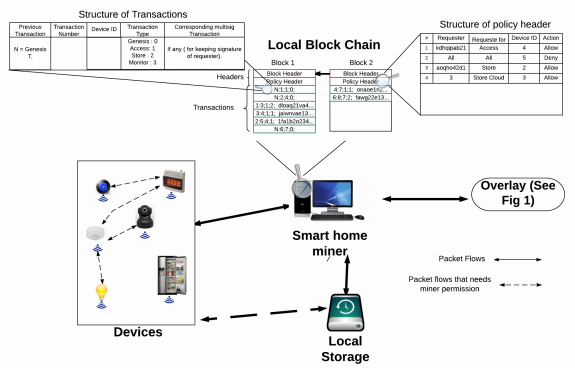
\includegraphics[height=0.5\textwidth]{pictures/home.png}
    \caption{Exemplo de blockchain aplicado em casa inteligente \cite{dorri2017blockchain}}
    \label{fig:home}
\end{figure}

Na figura \ref{fig:home} vemos um exemplo de como blockchain pode ser implementado em uma solução de automação residencial que utiliza IoT. Para aumentar a seguraça da casa inteligente todos os dispositivos conectados a internet estão protegidos contra solicitações maliciosas. Isto é feito limitando as transações aceitas as entidades com as quais cada dispositivo estabeleceu uma chave compartilhada. As transações recebidas da sobreposição são autorizadas antes de encaminhá-las para os dispositivos. Um contra argumento da efetividade dessa estrutura baseada em blockchain é que esse modelo apenas introduz um aumento marginal nos atrasos no processamento de transações em comparação com os produtos de gateway doméstico inteligentes existentes. Há sim também um único atraso adicional durante a inicialização para gerar e distribuir chaves compartilhadas. Em resumo, o adicional atrasos não são significativos e não afetam a disponibilidade de eletrodomésticos inteligentes. Para entender melhor esse modelo, e a forma genérica de como blockchain pode ser implementado em uma rede de qualquer escopo de dispositivos de internet das coisas, vamos separar a implementação em quatro pedaços: transações, blockchain local, minerador e armazenamento local.

As comunicações entre dispositivos locais ou nós de sobreposição são conhecido como transações. Um sistema genérico possui diversas transações, que só podem ser mais especificadas quando saímos do escopo da generalização e entramos no domínio do problema, como é o exemplo da casa inteligente, em que a transação da loja é gerada por dispositivos para armazenar dados, a transação de acesso é gerada por um SP (Service Provider) ou o dono da casa para acessar o armazenamento em nuvem e uma transação de monitor é gerada pelo proprietário da casa ou SPs para monitorar periodicamente um dispositivo em formação. Adicionar um novo dispositivo para a casa inteligente acontece através de uma transação gênesis e um dispositivo é removido através de uma transação de remoção. Todas as transações acima mencionadas usam uma chave compartilhada para proteger a comunicação. Lightweight Hashing é empregado para detectar qualquer alteração no conteúdo das transações durante a transmissão. Todas as transações de ou para a casa inteligente são armazenados em um local privado blockchain. Ou seja, se formos tomar isso em um aspecto genérico, as transações são responsáveis pela comunicação entre os diferentes atores envolvidos, sejam coisas conectadas a internet, um SP, a nuvem ou o usuário.

A blockchain privada local é mantida para acompanhar as transações e tem um cabeçalho de políticas para serem aplicas nos usuários para transações de entrada e saída. Começando com a transação gênesis, as transações de cada dispositivo são encadeadas juntos como um livro de registro imutável na blockchain. Cada bloco na blockchain local contém dois cabeçalhos, o de bloco e o de política. No cabeçalho do bloco tem o hash do bloco anterior para manter o BC imutável. O cabeçalho de política é usado para autorizar dispositivos e impor política de controle do proprietário sobre o sistema em que o blockchain foi aplicado (e.g. o dono da casa). O cabeçalho de política tem quatro parâmetros. O parâmetro ``Requester'' refere-se ao solicitante de chave pública na transação de sobreposição recebida. Para dispositivos locais, este campo é igual ao ``ID do dispositivo''. A segunda coluna no cabeçalho da política indica a ação solicitada na transação, que pode ser: armazenar para armazenar dados localmente, armazenar nuvem para armazenar dados no armazenamento em nuvem, acesso para acessar dados armazenados de um dispositivo e monitorar para acessar dados em tempo real de um dispositivo. A terceira coluna no cabeçalho da política é o ID do dispositivo dentro do sistema e , finalmente, a última coluna indica a ação que deve ser feita para a transação que corresponde com as propriedades anteriores. Além dos cabeçalhos, cada bloco contém um número de transações. Para cada transação, cinco parâmetros são armazenados na blockchain local. Os dois primeiros parâmetros são usados para encadear transações do mesmo dispositivo para o outro e identificar cada transação exclusivamente na blockchain. O ID do dispositivo correspondente da transação é inserido no terceiro campo. ``Tipo de transação'' refere-se a o tipo de transação que pode ser gênese, acesso, armazenamento ou monitorar transações. A transação é armazenada no quinto campo se vem da rede de sobreposição, caso contrário, este campo é mantido em branco. A blockchain local é mantido e gerenciado por um mineirador.

O mineirador do sistema é um dispositivo que processa de maneira centralizar transações de entrada e saída do sistema. O mineirador pode se integrar ao gateway de internet do sistema ou um dispositivo independente separado. O mineirador autentica, autoriza e monitora transações. Além disso, o mineirador também realiza as seguintes funções adicionais: gerar transações de gênese, distrubuição e atualização de chaves, alterar a estrutura de transações e formar e gerenciar o cluster. O minerador coleta todas as transações em um bloco e acrescenta o bloco inteiro ao blockchain. Para fornecer capacidade, o minerador gerencia um armazenamento local.

O armazenamento local é um dispositivo de armazenamento, por exemplo uma unidade de backup, que é usado por dispositivos para armazenar dados localmente. Este armazenamento pode ser integrado com o minerador ou pode ser um dispositivo separado. O armazenamento usa o método FIFO (first-in-first-out) para armazenar dados e armazena os dados de cada dispositivo como um ledger encadeado ao ponto de partida do dispositivo.

Esse é um modelo genérico que é capaz de descrever grande parte das implantações de sistemas blockchain como solução de segurança pra redes de internet das coisas. Outros modelos podem representar de maneira equivalente as características aqui demonstradas, com igual valor semântico.
\section{Projeto e Desenvolvimento De Uma Proposta}

Baseado nas possíveis soluções que foram tratadas na seção anterior, vamos usar o modelo genérico apresentado no trabalho de Casas Inteligentes \cite{dorri2017blockchain} para criar um modelo teórico que pode ser aplicado em qualquer implementação de soluções de segurança para internet das coisas utilizando a tecnologia blockchain, que apesar de ser uma tecnologia relativamente nova possui um poder promissor de paralelização que pode ser uma grande vantagem para redes IoT que contam com muitos dispositivos, mas cada um com poder de processamento pequeno individualmente.

Para isso, vamos considerar um modelo de Segurança em IoT utilizando Blockchain genérico como uma quádrupla $B = (T, Lpb, Hm, Ls)$, onde cada um dos elementos da estrutura é definido como:

\begin{itemize}
    \item $T$ é o conjunto de transações, as comunicações entre dispositivos locais ou nós de sobreposição. A definição desse conjunto é do domínio da aplicação, ou seja, depende do problema que a implementação da rede IoT resolve. Uma transação pode ser definida como uma tripla $t = (origin, destiny, message)$, onde $origin$ é o dispositivo que orina a transação, $target$ é o destino da comunicação e $message$ é o conteúdo trocado entre o par.
    
    \item $Lpb$ é a blockchain privada local (local blockchain, em inglês) é responsável por acompanhar as transações, e foi descrita em detalhes na seção anterior, sem perda de generalidade. Ela consta em um encadeamento de informações em forma de cabeçalhos de bloco e política.
    
    \item $Hm$ é o minerador local (home miner, em inglês), e é um dispositivo que processa de maneira centralizar transações de entrada e saída do sistema. Pode ser implementado de maneira física local ou pode ser um dispositivo virtual que está alocado em alguma núvem ou servidor, conforme a implementação demandar.
    
    \item $Ls$ é o armazenamento local (local storage, em inglês), e é o sistema de persistência de dados utilizado para que a blockchain possa ser utilizada de maneira contínua.
\end{itemize}{}

Para avaliar a qualidade do modelo que foi proposto por \cite{dorri2017blockchain}, no próprio trabalho de casas inteligentes foram feitas métricas para poder caracterizar melhor a solução implementada. As métricas são:

\begin{itemize}
    \item[] \textbf{Sobrecarga de tempo}: A Figura 2 mostra os resultados para o tempo de overhead. O projeto baseado em blockchain consome mais tempo para processar pacotes, comparado a implementação original da rede IoT estudada. Isso pode ser atribuído às operações adicionais de criptografia e hashing. No pior caso em uma transação de consulta, a sobretaxa adicional causada pelo método é 20 ms, o que ainda pode ser considerada uma sobrecarga pequena em vista a vantagem trazida pela implementação utilizando blockchain.
    \begin{figure}[H]
        \centering
        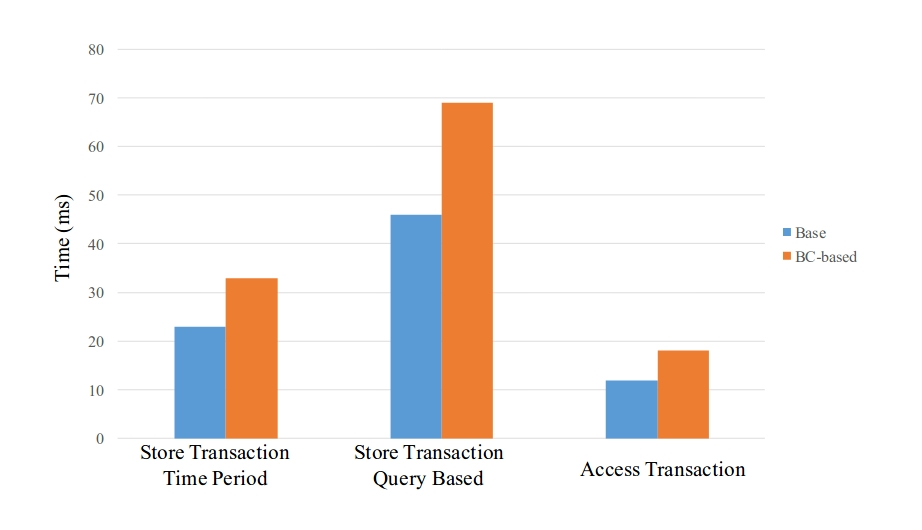
\includegraphics[width=0.8\textwidth]{pictures/results1.jpg}
        \caption{Gráfico dos dados de sobrecarga}
        \label{fig:results1}
    \end{figure}{}
    
    \item[] \textbf{Consumo de Energia}: A Figura 3 descreve os resultados de consumo de energia. Como é evidente, o projeto baseado em blockchain aumenta o consumo de energia em 0,07 (mj). A tabela na parte inferior da Figura 3 descreve o consumo de energia para as 3 tarefas centrais executadas pelo minerador: CPU, transmissão (Tx) e escuta (Lx). O consumo de energia por CPU aumentou em torno de 0,002 (mj) mp projeto devido a criptografia e hashing. A transmissão de pacotes de dados mais longos dobrou o consumo de energia de transmissão da solução utilizando em blockchain em comparação com o método que não usava. As baixas despesas gerais introduzidas pela solução que utiliza blockchain para segurança em internet das coisas superam significativamente o que não utiliza blockchain dados os significativos benefícios de segurança e privacidade oferecidos em troca de um custo não tão alto de energia.
    
    \begin{figure}[H]
        \centering
        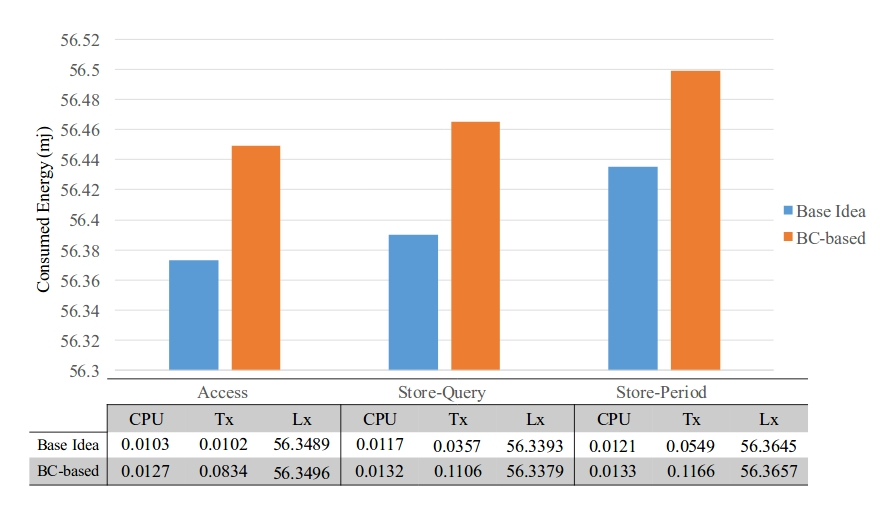
\includegraphics[width=0.8\textwidth]{pictures/results2.jpg}
        \caption{Gráfico dos dados de consumo de energia}
        \label{fig:my_label}
    \end{figure}{}
\end{itemize}{}

\section{Conclusões e Trabalhos Futuros}

A ideia desse trabalho foi fazer uma revisão sistemática da literatura até então existente, apresentação de um modelo genérico para implementar a solução proposta e ter uma discussão dos benefícios, desafios e do futuro de segurança em internet das coisas, em específico do uso de técnicas da blockchain para tratar desses problemas. 

O modelo apresentado, que descreve os sistemas apresentados na revisão sistemática, pode servir como base para diversas implementações de sistemas de segurança para redes de internet das coisas utilizando blockchain. Apesar de servir muito bem, e já ter sido provado eficiente através de implementações iniciais, ainda existem problemas a serem resolvidos na área como um todo. A maior dificuldade, sem dúvida, é o alto consumo energético, derivado do requisito computacional que os algoritmos de segurança blockchain requerem, além da memória utilizada. Apesar do resultado da implementação específica ter sido muito satisfatório tanto em custo computacional quanto em custo energético, mais estudo na área é necessário para poder se chegar a conclusões concretas e que abranjam de maneira mais geral modelos segurança para redes do tipo. Como os sensores e microprocessadores utilizados pelas ``coisas'' nas redes de IoT serem muito simples, com baixo potencial computacional, baixa memória e necessidade de baixo consumo energético por questões térmicas, muito dos algoritmos de blockchain precisam ser revistos para que esse tipo de solução se torne simples de ser implantada e comum de ser vista nas redes domésticas, industriais e científicas.

O principal trabalho discutido em nossa revisão, e que foi utilizado como base para montarmos uma proposta concreta de solução genérica de segurança para internet das coisas utilizando blockchain \cite{dorri2017blockchain}, mostra como é possível fazer implementações do tipo, pois no trabalho realmente foi feita uma rede completa de internet das coisas para que os testes fossem realizados, tanto com blockchain quanto sem blockchain. Apesar do exemplo com blockchain ter apresentado resultados espetaculares com um custo de energia bem reduzido e tempo de resposta adicional quase desconsideráveis, mesmo que maior do que a implementação sem blockchain, que em questão de segurança era muito inferior devido a natureza simples das verficações de segurança e confiabilidade da rede, a replicação em larga escala do mesmo modelo ainda assim poderia trazer problemas por conta de um crescimento linear do custo. Mesmo assim, esse trabalho é pioneiro na área de otimização do tipo de solução apresentada, e tende a ser um tipo de trabalho a se repetir em novas esferas, com contextos diferentes e implementações ainda mais otimizadas que vão tornar possível a indústria aplicar esse tipo de solução a qualquer rede de coisas inteligentes a serem vendidas para o usuário final.

Em nosso trabalho apresentamos um modelo genérico, que possui certa validação mas que ainda pode ser aprimorado e testado arduamente para conseguir dados mais objetivos e relevantes para que a proposta como um todo se concretize como uma solução válida e implementável para redes de diversos tamanhos. Caso isso não aconteça, é certo que para determinados tipos e tamanhos de redes de internet das coisas o modelo funciona, então mesmo assim pode ser utilizado, apenas em empreitadas específicas e talvez reduzidas.

Portanto, os trabalhos futuros devem almejar não só a corretude da solução proposta, com modelos que já foram apresentados como funcionais por trabalhos anteriores, mas também focar na otimização das soluções para que tenham necessidade de menor custo computacional e consumo energético, para que em aplicações de larga escala a solução utilizando blockchain continue viável, mesmo com possivelmente milhões de coisas inteligentes interconectadas. Uma alternativa para essa solução é investir em soluções distribuídas, onde a computação pode ser distribuída de maneira eficiente através de algoritmos de distribuição de carga entre os diversos microprocessadores da rede IoT, extraindo o máximo potencial que essa tecnologia tem a oferecer com sua natureza de muitos dispositivos com pouco potencial de computação individual.

Além do avanço no trabalho atual como citado no parágrafo anterior, a arquitetura apresentada, bem como as contribuições que ela traz para a segurança em internet das coisas mesclando o crescente uso de controladores inteligentes com conceitos como blockchain, podem ser ainda mais mesclados com conceitos avançados de computação, IoT ou segurança. Um exemplo claro disso é a possibilidade de aplicar a técnica de Fog computing no modelo apresentado. Essa adição está fora do escopo do trabalho realizado, mas combina perfeitamente com a ideia de reduzir custo computacional de maneira geral na rede de internet das coisas e nesse caso específico para reduzir o custo computacional da implementação do Blockchain em um ambiente com diversos sensores transmitindo um grande volume de dados constantemente.

Por último, vale ressaltar a importância da transparência e da comunicação humana além das estratégias de segurança adotada. É crucial que o consumidor saiba que tipo de dados estão sendo coletados, e que tipo de sensores existem nos dispositivos inteligentes instalados em sua casa para que o relacionamento entre o consumidor e a rede utilizada seja saudável, despertando não só o interesse comercial com um aproveito unilateral por parte das empresas que provém esse tipo de serviço. Aviso da escolha, do mecanismo de acesso e da precisão da informação recolhida, políticas efetivas de minimização dos dados coletados e prestação de contas das medidas e falhas de segurança nos dispositivos são alguns fundamentos que tem se mostrado tendência por empresas que presam por um relacionamento saudável com o consumidor.


% ----------------------------------------------------------
% Referências bibliográficas
% ----------------------------------------------------------
\bibliography{abntex2-modelo-references}


\end{document}
